\documentclass[12pt, openright, a4paper, brazil, english, french, spanish, bibjustif, openany, oneside]{abntex2}

\usepackage{cmap}				% Mapear caracteres especiais no PDF
\usepackage{ifthen}				% Mapear caracteres especiais no PDF
\usepackage{setspace}				% Mapear caracteres especiais no PDF
\usepackage{lmodern}		
\usepackage[T1]{fontenc}	
\usepackage[utf8]{inputenc}
\usepackage{lastpage}
\usepackage{enumitem}	
\usepackage{indentfirst}	
\usepackage{color}			
\usepackage{graphicx}
\usepackage[table]{xcolor}
\usepackage{tabularx}
\usepackage{booktabs}
\usepackage{enumerate}		
\usepackage{microtype} 		
\usepackage{multicol}
\usepackage{multirow}
\usepackage{lipsum}
\usepackage{booktabs}				
\usepackage{bold-extra}				% Mapear caracteres especiais no PDF
\usepackage[final]{pdfpages}

\usepackage[brazilian,hyperpageref]{backref}	 % Paginas com as citações na bibl
\usepackage[alf]{abntex2cite}	% Citações padrão ABNT

\usepackage[small]{caption}


\newtheorem{teo}{Teorema}
	 
%
%\titulo{Usando o Scratch como ferramenta interdisciplinar através da programação}
%\autor{Sérgio Luís Soares Almeida \\ Matrícula 18/0006410}
%\local{Brasília}
%\data{2019}
%\instituicao{%
%  Universidade de Brasília -- UnB
%  \par
%  Departamento de Matemática
%  \par
% PROFMAT}
%\tipotrabalho{Estudo de Artigo}

%\definecolor{black}{RGB}{0.0,0.0,0.0}


%\makeatletter

%\preambulo{Scratch no ensino de Matemática}

%\hypersetup{pdftitle={\@title}, pdfauthor={\@author}, pdfsubject={\imprimirpreambulo}, pdfcreator={LaTeX with abnTeX2}, pdfkeywords={abnt}{latex}{abntex}{abntex2}{relatório técnico}, colorlinks=true, linkcolor=black, citecolor=black, filecolor=black, urlcolor=black, bookmarksdepth=4}
%\makeatother

%\setlength{\parindent}{1.3cm}


%\setlength{\parskip}{0.2cm}  


%\makeindex

%=============================================================================================
%teste de apendice
\renewcommand\appendixname{APÊNDICE}
\renewcommand\appendixpagename{APÊNDICE}
%=============================================================================================


%informações do título

\titulo{Usando o Scratch como ferramenta interdisciplinar através da programação}
\autor{Sérgio Luís Soares Almeida}
\local{Brasília}
\data{\the\year}
\orientador[Orientadora:]{Prof$^{\underline{a}}$. Dr$^{\underline{a}}$. Tatiane da Silva Evangelista}
\coorientador{}
\instituicao{%
  Universidade de Brasília - UnB
  \par
  Departamento de Matemática - MAT
  \par
  PROFMAT - SBM}
\tipotrabalho{Dissertação de Mestrado}
% O preambulo deve conter o tipo do trabalho, o objetivo, 
% o nome da instituição e a área de concentração 
\preambulo{Dissertação apresentada ao Departamento de Matemática da Universidade de Brasília, como parte dos requisitos do Programa de Mestrado Profissional em Matemática em Rede Nacional - PROFMAT, para obtenção do grau de Mestre.}


%Novas configurações enviadas pelo Vinícius

\makeatletter
\newcommand*{\textoverline}[1]{$\overline{\hbox{#1}}\m@th$}
\makeatother
% ---
% Configurações do pacote backref
% Usado sem a opção hyperpageref de backref
\renewcommand{\backrefpagesname}{Citado na(s) página(s):~}
% Texto padrão antes do número das páginas
\renewcommand{\backref}{}
% Define os textos da citação
\renewcommand*{\backrefalt}[4]{
	\ifcase #1 %
		Nenhuma citação no texto.%
	\or
		Citado na página #2.%
	\else
		Citado #1 vezes nas páginas #2.%
	\fi}%
% ---

\renewcommand{\imprimircapa}{%
  \begin{capa}%
    \center
    \begin{minipage}[t][1cm][c]{0.2\textwidth}
        
\includegraphics[scale=0.6,keepaspectratio=true]{unb.png}
    \end{minipage}
    \begin{minipage}[t][1cm][c]{0.5\textwidth}
        \begin{center}
        Universidade de Brasília \\
        Instituto de Ciências Exatas \\
        Departamento de Matemática \\
        Programa de Mestrado Profissional\\
        em Matemática em Rede Nacional
        \end{center}
    \end{minipage}
    \begin{minipage}[t][1cm][c]{0.2\textwidth}
        
\includegraphics[scale=0.6,keepaspectratio=true]{profmat.jpg}
    \end{minipage}

    \vspace*{1cm}

    \vfill
    \begin{center}
    \ABNTEXchapterfont\bfseries\LARGE\imprimirtitulo
    \end{center}
    \vfill

    {\ABNTEXchapterfont\large\imprimirautor}

    \vspace*{2cm}

    \large\imprimirlocal

    \large\imprimirdata

    \vspace*{1cm}
  \end{capa}
}

\newcounter{obmepquestion}

\newenvironment{enunciado}
{
    \stepcounter{obmepquestion}
    \bfseries
}
{
}

\newenvironment{analise}[8]
{
    \vspace{0.2in}
    \noindent
    \begin{minipage}[c][4cm][c]{0.55\textwidth}
        
    \begin{small}
    \begin{center}
    \bfseries{\scshape{Análise do Item \arabic{obmepquestion}}}
    \end{center}
    \end{small}

    \begin{tiny}
    \begin{tabular}{cccccc}
        \toprule
        \rowcolor{blue!20}
        Questão & Gabarito & Dificuldade & \multicolumn{2}{c}{Índice D} &
            Bisserial \\
        #1 & \multicolumn{2}{c}{#2} & #3 \\
        \rowcolor{blue!20}
        \multicolumn{3}{c}{Acerto: 27\% maiores notas} &
        \multicolumn{3}{c}{Acerto: 27\% menores notas} \\
        \multicolumn{3}{c}{#4} &
        \multicolumn{3}{c}{#5} \\
        \rowcolor{blue!20}
        $r_b(A)$ & $r_b(B)$ & $r_b(C)$ & $r_b(D)$ & $r_b(E)$ & $r_b()$ \\ 
        #6 \\
        \rowcolor{blue!20}
        $p(A)$ & $p(B)$ & $p(C)$ & $p(D)$ & $p(E)$ & $p()$ \\ 
        #7 \\
        \bottomrule
    \end{tabular}
    \end{tiny}
    \end{minipage}
    \begin{minipage}[c][4cm][c]{0.45\textwidth}
        \includegraphics[scale=0.25,keepaspectratio=true]{#8}
    \end{minipage}
}
{
    \vspace{0.2in}
}


\newcommand{\alternativas}[6]
{
    \vspace{0.2in}
    \noindent
    \begin{minipage}[t][1cm][c]{0.5\textwidth}
    \begin{flushleft}
    \begin{enumerate}[itemsep=-2mm, label=\Alph*)]
        \item #1
        \item #2
        \item #3
        \item #4
        \item #5
    \end{enumerate}
    \end{flushleft}
    \end{minipage}
    \begin{minipage}[t][1cm][c]{0.5\textwidth}
    \ifthenelse{\equal{#6}{}}{}{
        \includegraphics[scale=0.6,keepaspectratio=true]{#6}
    }
    \end{minipage}
    \vspace{0.5in}
}

% ---
% Configurações de aparência do PDF final

% alterando o aspecto da cor azul
\definecolor{blue}{RGB}{41,5,195}

% informações do PDF
\makeatletter

\hypersetup{
     	%pagebackref=true,
		pdftitle={\@title}, 
		pdfauthor={\@author},
    	pdfsubject={\imprimirpreambulo},
	    pdfcreator={LaTeX with abnTeX2},
		pdfkeywords={abnt}{latex}{abntex}{abntex2}{trabalho acadêmico}, 
		colorlinks=true,       		% false: boxed links; true: colored links
    	linkcolor=black,          	% color of internal links
    	citecolor=black,        		% color of links to bibliography
    	filecolor=black,      		% color of file links
		urlcolor=black,
		bookmarksdepth=4
}
\makeatother
% --- 

% --- 
% Espaçamentos entre linhas e parágrafos 
% --- 

% O tamanho do parágrafo é dado por:
\setlength{\parindent}{1.3cm}

% Controle do espaçamento entre um parágrafo e outro:
\setlength{\parskip}{0.2cm}  % tente também \onelineskip

\begin{document}






\selectlanguage{brazil}


\frenchspacing 
\imprimircapa
\imprimirfolhaderosto*

%novos elementos do documento
% FICHA CATALOGRÁFICA

\begin{fichacatalografica}
	\vspace*{\fill}					% Posição vertical
	\hrule							% Linha horizontal
	\begin{center}					% Minipage Centralizado
	\begin{minipage}[c]{12.5cm}		% Largura

	\imprimirautor
	
	\hspace{0.5cm} \imprimirtitulo  / \imprimirautor. --
	\imprimirlocal, \imprimirdata-
	
	\hspace{0.5cm} \pageref{LastPage} p. : il. (algumas color.) ; 30 cm.\\
	
	\hspace{0.5cm} \imprimirorientadorRotulo~\imprimirorientador\\
	
	\hspace{0.5cm}
	\parbox[t]{\textwidth}{\imprimirtipotrabalho~--~\imprimirinstituicao,
	\imprimirdata.}\\
	
	\hspace{0.5cm}
		1. Palavra Chave 1.
		2. Palavra Chave 2.
		I. Nome do Orientador.
		II. Universidade de Brasília.
		III. PROFMAT - SBM.
		IV. Título XYZ\\ 			
	
	\hspace{8.75cm} ?CDU XYZ 02:141:005.7?\\
	
	\end{minipage}
	\end{center}
	\hrule
\end{fichacatalografica}

% FOLHA DE APROVAÇÃO

\begin{folhadeaprovacao}

\begin{center}
 Universidade de Bras\'ilia \\
 Instituto de Ci\^encias Exatas \\
 Departamento de Matem\'atica
\end{center}
\begin{center}
    \vspace{0.3cm}
 \LARGE{\textbf{\imprimirtitulo}}
    \vspace{0.3cm}
\end{center}
\begin{center}
 por \\
    \vspace{0.5cm}
 \LARGE{\textbf{\imprimirautor}} *
\end{center}

    \vspace{0.5cm}
\noindent Disserta\c c\~ao apresentada ao Departamento de Matem\'atica da Universidade de Bras\'ilia,
como parte dos requisitos do ``Programa'' de Mestrado Profissional em Matem\'atica em Rede 
Nacional - PROFMAT, para obten\c c\~ao do grau de 
\begin{center}
    \vspace{0.2cm}
 \LARGE{\textbf{MESTRE}}\\
    \vspace{0.5cm}
 Bras\'ilia, 29 de maio de 2020
\end{center}

    \vspace{1.5cm}
\noindent {Comiss\~ao Examinadora:}

\vspace*{8mm}

\textoverline{\phantom{xxxxxxx} \imprimirorientador - MAT/UnB (Orientadora)\phantom{xxxxxxx}  }

\vspace*{1cm}

\textoverline{\phantom{xxxxxxx} Prof. Dr. Membro 1 - MAT/UnB (Membro) \phantom{xxxxx} }

\vspace*{1cm}

\textoverline{\phantom{xxxxxxx} Prof. Dr. Membro 2 - SEEDF (Membro)\phantom{xxxxxxx}  }

\vspace*{1cm}

\vspace*{1cm}

\end{folhadeaprovacao}

%folha dedicatória

\begin{dedicatoria}
   \vspace*{\fill}
   \centering
   \noindent
    \textit{Texto da dedicatória.}\vspace*{\fill}
\end{dedicatoria}

%folha agradecimentos

\begin{agradecimentos}

Texto do agradecimento.

\end{agradecimentos}

%folha epigrafe

\begin{epigrafe}
    \vspace*{\fill}
	\begin{flushright}
		\textit{\lq\lq Citação \rq\rq\\ Autor}
	\end{flushright}
\end{epigrafe}

%folha resumo

\begin{resumo}

Texto do resumo.

 \vspace{\onelineskip}
    
 \noindent
 \textbf{Palavras-chaves}: palavras. chaves. separadas. por. pontos.
\end{resumo}

%folha abstract

\begin{resumo}[Abstract]
 \begin{otherlanguage*}{english}

Texto do abstract.

  \vspace{\onelineskip}
 
   \noindent 
 \textbf{Key-words}: palavras. chaves. separadas. por. pontos.
 \end{otherlanguage*}
\end{resumo}



%novas configurações de capa e contracapa
\pdfbookmark[0]{\listfigurename}{lof}
\listoffigures*
\cleardoublepage

\pdfbookmark[0]{\listtablename}{lot}
\listoftables*
\cleardoublepage

\pdfbookmark[0]{\contentsname}{toc}
\tableofcontents*
\cleardoublepage
% ----------------------------------------------------------
% ELEMENTOS TEXTUAIS
% ----------------------------------------------------------
\textual

%\ABNTEXchapterfont
%\pdfbookmark[0]{\contentsname}{toc}
%\tableofcontents*
%\cleardoublepage
%\textual

\chapter*[Introdução]{Introdução}
\addcontentsline{toc}{chapter}{Introdução}

Fazer introdução


\chapter{Pensamento Computacional}

O termo \textit{``computational thinking''} (pensamento computacional) passou a ser mais discutido a partir do artigo de Jeannette M. Wing em 2006, onde afirma que ``o pensamento computacional baseia-se no poder e nos limites dos processos de computação, sejam eles executados por um ser humano ou por uma máquina''\cite{wing}. Ainda, segundo Wing:

\begin{citacao}

``O pensamento computacional é uma habilidade fundamental para todos, não apenas para cientistas das computação. À leitura, escrita e aritmética, devemos acrescentar o pensamento computacional à capacidade analítica de cada criança'' \cite{wing}

\end{citacao}




No entanto o termo pensamento computacional não é definido em termos precisos. Em dois workshops sobre o âmbito e a natureza do pensamento computacional, patrocinados pela \textit{National Academy of Sciences} dos Estados Unidos da América, em 2009 e 2011, a \textit{National Research Council} publicou:

\begin{citacao}

``Os debates realizados no Workshop de fevereiro de 2009 não chegaram a um acordo geral entre os participantes sobre o conteúdo preciso de pensamento computacional, e muito menos a sua estrutura. No entanto, a falta de desacordo explícito sobre seus membros poderia ser entendida como refletindo uma intuição compartilhada entre os participantes do workshop que o pensamento computacional, como um modo de pensamento, tem o seu próprio caráter distintivo'' \cite{NRC}

\end{citacao}

As organizações \textit{International Society for Technology in Education} (ISTE) e a \textit{American Computer Science Teachers Association} (CSTA) trabalharam com pesquisadores da Ciência da Computação e das áreas de Humanas e construiram uma definição para o pensamento computacional pautada em elementos objetivos que pudesse nortear as atividades realizadas na Educação Básica identificando os seguintes conceitos: coleta de dados, análise de dados, representação de dados, decomposição do problema, abstração, algoritmos, automação, paralelização e simulação. Assim o pensamento computacional é definido como:

\begin{citacao}

``Pensamento computacional é um processo de solução de problemas que inclui (mas não está limitado a) as seguintes características: Formular problemas de uma forma que nos permita usar um computador e outras ferramentas para ajudar a resolvê-los; Organizar e analisar logicamente os dados; Representar dados através de abstrações, como modelos e simulações; Automatizar soluções por meio de pensamento algorítmico; Identificar, analisar e implementar possíveis soluções com o objetivo de alcançar a combinação mais eficientes e eficaz de etapas e recursos; Generalizar e transferir esse processo de solução de problemas para uma ampla variedade de problemas.''\cite{iste/csta}

\end{citacao}

Estas características podem ser melhor compreendidas ao fazer um estudo mais detalhado de cada uma delas:

\begin{itemize}
\item \textbf{Formular problemas de uma forma que nos permita usar um computador e outras ferramentas para ajudar a resolvê-los}

Ao enfrentar situações problemas, as primeiras análises a serem feitas são: como podemos resolvê-las, que ferramentas podem ser utilizados ou ainda quem é o mais qualificado a resolvê-las. Ao encontrar respostas as essas análises, pode-se definir quais estruturas devem ser usadas para cada situação problema.

\item \textbf{Organizar e analisar logicamente os dados}

A situação problema inicial será subdividida em situações problemas menores de tal forma que a análise dos dados determinará a ordem em que cada uma dessas subdivisões deverão ser resolvidas.

\item \textbf{Representar dados através de abstrações, como modelos e simulações}

Com a subdivisão da situação problema inicial, verificar quais características são repetidas em cada subdivisão e ao reconhecer esses padrões destacar o que é mais relevante para a construção de modelos e para se fazer abstrações relativas para definir melhor a solução.

\item \textbf{Automatizar soluções por meio de pensamento algorítmico}

Criar instruções claras, detalhadas de como cada subdivisão da situação problema deve ser resolvida e assim criar algoritmos de soluções que podem ser traduzidos e replicados quantas vezes forem necessários.

\item \textbf{Identificar, analisar e implementar possíveis soluções com o objetivo de alcançar a combinação mais eficientes e eficaz de etapas e recursos}

Neste estágio, a análise é feita com base nas instruções dadas, verificando se existem redundâncias, se existem soluções mais práticas e eficazes para cada subdivisão e se a solução é realmente viável.

\item \textbf{Generalizar e transferir esse processo de solução de problemas para uma ampla variedade de problemas}

Com a solução encontrada, analisar se a estrutura encontrada pode ser estendida para outras situações problemas semelhantes, aumentando assim a abrangência de todo o processo.

\end{itemize}

Os pesquisadores do ISTE/CSTA observam ainda que essas habilidades são ``apoiadas e reforçadas por uma série de disposições ou atitudes que são dimensões essenciais do pensamento computacional'' assim como ``confiança em lidar com a complexidade, persistência em trabalhar com problemas difíceis, tolerância para a ambiguidade e capacidade de lidar com problemas abertos''\cite{iste/csta}.

Essas características deixam transparecer que o pensamento computacional é uma habilidade que qualquer pessoa deveria ter, independentemente da área de conhecimento ou atividade profissional já que não envolve apenas os conceitos da Computação pois também agrega práticas de projetar sistemas, entender o comportamento humano e o pensamento crítico \cite{wing}.

Não devemos confundir ``Pensamento Computacional'' com ``Alfabetismo Digital'', pois este último é a simples aptidão de manusear aplicativos eletrônicos. As novas gerações que ingressam hoje na escola e que estão imersos na linguagem digital dos computadores, vídeo games e da Internet são considerados "nativos digitais", mas Mitch Resnick (2012) questiona a fluência digital destes jovens e explica que embora estes jovens tenham nascidos em um ambiente tecnológico e demonstrem muita experiência e facilidade em interagir com tecnologias, não tem esta mesma habilidade para criar e se expressar utilizando essas novas tecnologias, comparando este jovem com alguém que sabe ler, mas não sabe escrever.

O desenvolvimento do pensamento computacional no jovens exige que a formação do professor também passe por mudanças, não apenas reproduzindo os conhecimentos através de aplicativos, mas também resolvendo problemas através das tecnologias. Como disse Brackmann (2017):

\begin{citacao}

``A integração das TICs no currículo e na aprendizagem no campo da sua formação inicial é um desafio, pois durante o processo de tornar o pensamento computacional como uma competência fundamental para o século XXI, os professores também devem obrigatoriamente se aproximar dessas tecnologias e refletir dentro da sua área como a diversidade de conceitos, teorias, modelos e práticas podem ser aplicados dentro de sua disciplina de forma abrangente.'' \cite{brac}. 

\end{citacao}


O Pensamento Computacional pode e deve ser inserido na Educação básica através das disciplinas já existentes e que estão de acordo com a Base Nacional Comum Curricular - BNCC, de tal forma que o seu uso possa ser incentivado em várias disciplinas para que atinja um público cada vez maior. O CSTE/ISTE (2009) também realizou um levantamento com diversas propostas de adoção de forma Pluri, Multi e Transdiciplinar, de forma que BRACKMANN (2017) as combinou através de duas tabelas.

A tabela \ref{tab1} mostra sugestões de inserção do Pensamento Computacional nas disciplinas de Matemática e Ciências.

\newpage

\begin{table}[ht]
        \centering
        \caption{Sugestões de inserção do PC nas disciplinas de Matemática e Ciências \label{tab1}}
                
        \begin{tabular}{ >{\centering\arraybackslash}m{3cm} >{\centering\arraybackslash}m{5.5cm} >{\centering\arraybackslash}m{6cm}}
            \toprule
            \textbf{Conceitos de PC} & \textbf{MATEMÁTICA} & \textbf{CIÊNCIAS} \\
            \midrule
            \textbf{Coleção de Dados} & Encontrar uma fonte de dados de uma experiência, por exemplo: cara ou coroa, lançar dados & Coletar dados de um experimento \\
            \midrule
            \textbf{Análise de Dados} & Contar a ocorrência de jogadas, lançamentos de dados e análise de resultados & Analisar dados de um experimento  \\
            \midrule
            \textbf{Representação de Dados} & Utilizar gráfico de barras e de pizza para representação de dados. Usar conjuntos, listas, representações gráficas, etc. para a visualização de informações & Resumir dados de um experimento \\
            \midrule
            \textbf{Decomposição de Problemas} & Aplicar ordem de operadores & Realizar uma classificação de espécies \\
            \midrule
            \textbf{Abstração} & Usar variáveis na álgebra. Estudar funções de álgebra através de comparação em computadores. & Construir um modelo de uma entidade física \\
            \midrule
            \textbf{Algoritmos e Procedimentos} & Realizar divisões longas, fatorar & Criar um procedimento experimental \\
            \midrule
            \textbf{Automação} & Utilizar ferramentas como: Geometer, Sketch Pad, Star Logo, linhas de código em Python, etc. & Usar simulação de dados \\
            \midrule
            \textbf{Paralelismo} & Resolução de sistemas lineares. Multiplicação de matrizes. & Realizar experimentos com diferentes parâmetros simultaneamente. \\
            \midrule
            \textbf{Simulação} & Desenhar uma função em um plano cartesiano e modificar os valores das variáveis & Simular os movimentos do Sistema Solar \\
            \bottomrule
        \end{tabular}
        \fonte{BRACKMANN, 2017}
    \end{table}

\newpage

Na tabela \ref{tab2}, BRACKMANN (2017) mostra que o Pensamento Computacional também pode ser aplicado em outras disciplinas, com sugestões de inserção nas disciplinas de Estudos Sociais, Linguagens e Artes. 

\begin{table}[h]
        \centering
        \caption{Sugestões de inserção do PC nas disciplinas de Estudos Sociais, Linguagens e Artes \label{tab2}}
                
        \begin{tabular}{ >{\centering\arraybackslash}m{3cm} >{\centering\arraybackslash}m{5.5cm} >{\centering\arraybackslash}m{6cm}}
            \toprule
            \textbf{Conceitos de PC} & \textbf{ESTUDOS SOCIAIS} & \textbf{LINGUAGENS E ARTES} \\
            \midrule
            \textbf{Coleção de Dados} & Estudar estatísticas de guerras ou dados populacionais  & Identificar padrões em diferentes tipos de frases \\
            \midrule
            \textbf{Análise de Dados} & Identificar as tendências dos dados estatísticos & Representar padrões de diferentes tipos de frases  \\
            \midrule
            \textbf{Representação de Dados} & Resumir e representar tendências & Escrever um rascunho \\
            \midrule
            \textbf{Abstração} & Resumir fatos. Deduzir conclusões dos fatos & Uso de metáforas e analogias. Escrever uma história com diversas vertentes \\
            \midrule
            \textbf{Algoritmos e Procedimentos} & - & Escrever instruções \\
            \midrule
            \textbf{Automação} & Usar planilhas eletrônicas & - \\
            \midrule
            \textbf{Paralelismo} & - & Utilizar o corretor ortográfico \\
            \midrule
            \textbf{Simulação} & Incentivar com jogos que utilizem bases históricas & Encenação de uma história \\
            \bottomrule
        \end{tabular}
        \fonte{BRACKMANN, 2017}
    \end{table}

Assim percebemos como o desenvolvimento do Pensamento Computacional nos jovens pode ser importante na aprendizagem de qualquer disciplina desde que usado corretamente e com objetivos claros e bem definidos. Desta forma a inserção do Pensamento Computacional em sala de aula irá proporcionar a construção de novos conhecimentos e de novas abordagens para problemas do nosso dia-a-dia.


\chapter{Objetos de Aprendizagem}

Os Objetos de Aprendizagem podem ser um grande aliado do professor como ferramenta de aprendizagem e de revisão de conceitos em vários conteúdos e propostas de ensino. A metodologia e o planejamento de suas aplicações são fatores determinantes para o sucesso da aprendizagem e para o desenvolvimento de estratégias para resolução de problemas, o seu uso deve estar previamente ligado aos objetivos do conteúdo e da aprendizagem que se quer alcançar. Podem ser de qualquer mídia ou formato, como uma apresentação em stop motion (animação quadro-a-quadro) ou uma simulação.

Não há um consenso sobre o conceito de Objetos de Aprendizagem, cada autor define de acordo com uma concepção própria levando em consideração a utilidade e importância do Objeto para o ensino e a aprendizagem, desta forma, é importante que o conceito de um Objeto de Aprendizagem esteja de acordo com o objetivo do estudo e do planejamento do momento de aprendizagem. Entretanto, uma definição de Objetos de Aprendizagem significativa é dada por Tarouco (2003):


\begin{citacao}

``Um Objeto de Aprendizagem é qualquer recurso, suplementar ao processo de aprendizagem, que pode ser reusado para apoiar a aprendizagem, termo geralmente aplicado a materiais educacionais projetados e construidos em pequenos conjuntos visando a potencializar o processo de aprendizagem onde o recurso pode ser utilizado.''\cite{tarouco}

\end{citacao}

Nesta definição devem ser destacadas as palavras ``recurso'', ``suplementar'' e ``reusado'', pois um Objeto de Aprendizagem não deve ser o objeto da aprendizagem mas um recurso que o aluno possa utilizar para ajudá-lo a alcançar a aprendizagem do conteúdo previamente exposto dentro dos objetivos pretendidos e que podem ser reutilizados não só para um conteúdo específico mas também em conjunto com outros Objetos de Aprendizagem que podem ser combinados e recombinados dentro de um mesmo contexto e com conteúdos relacionados.

A construção de um objeto de aprendizagem envolve um planejamento prévio que possa responder às perguntas:

\begin{itemize}
\item Quais os objetivos a serem alcançados?
\item Qual o público alvo, suas habilidades, seu conhecimento prévio?
\item Qual a interface a ser usada?
\item Quais ferramentas serão utilizadas para a sua construção?
\item O Objeto de Aprendizagem tem relação com mais de um conteúdo e pode ser recombinado?
\end{itemize}

Ao responder essas perguntas os objetos de aprendizagem construídos serão mais eficientes e com maior capacidade de serem reutilizados e recombinados com outros conteúdos.



\chapter{Apresentando o Scratch}

 O Scratch é uma linguagem de programação feita por blocos lógicos capaz de integrar sons e imagens em histórias interativas, jogos e animações entre outros programas interativos desenvolvidos pelo usuário de forma intuitiva e sem o conhecimento prévio de outras linguagens de programação. Foi idealizado por Mitchel Resnick para pessoas com idades a partir de 8 anos e criado em 2007 pelo Lifelong Group, no MIT (Instituto de Tecnologia de Massachussets) Media Lab, onde continua sendo desenvolvido e moderado.  Hoje é usado em mais de 150 países e está disponível em mais de 40 idiomas.
 
 O Scratch é bastante acessível já que usa uma interface gráfica em que os programas são construidos através de blocos lógicos auto-encaixantes lembrando a montagem de um puzzle. A sua interface é de fácil compreensão (vide figura \ref{scr1}) e o uso de suas ferramentas muito intuitivas e sem complicações, possuindo três principais áreas:
 
\begin{enumerate}
\item Nesta área estão armazenados os blocos de comando, organizados a partir da sua funcionalidade.
\item A área de comandos a serem seguidos, onde os blocos serão encaixados
\item Palco ou simulador do Ecrã, onde se pode ver a simulação ou execução dos comandos.
\end{enumerate}

\begin{figure}[h]

    \center

    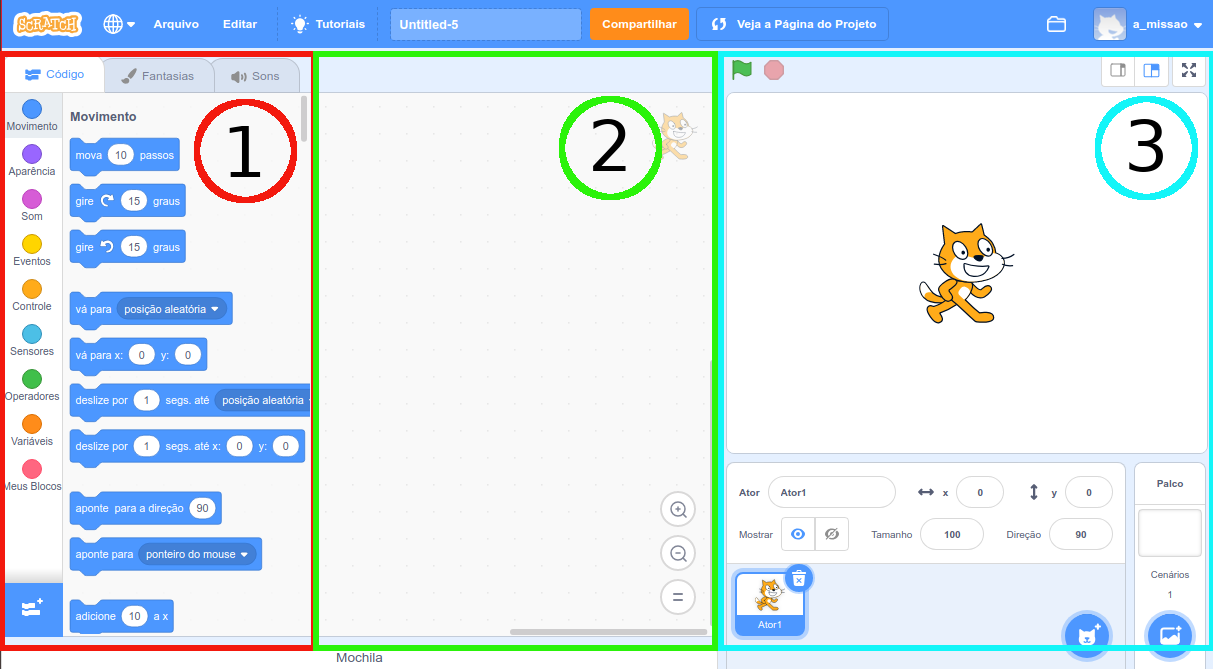
\includegraphics[width=15cm]{scratch1.png}
    \caption{interface do Scratch \label{scr1}}
    
\end{figure}

\newpage

A primeira área, ou área de blocos de comando (\ref{scr2}), estão os comandos que podem ser usados na programação a ser realizada. Esses comandos estão subdivididos em categorias a partir de suas funcionalidades, como movimento, aparência, som, etc.

\begin{figure}[h]

    \center

    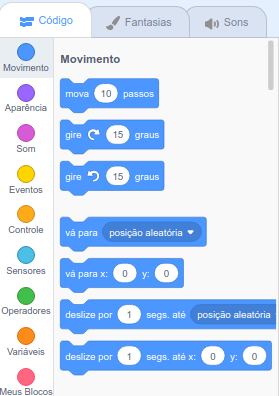
\includegraphics[height=7cm]{scratch2.png}
    \caption{área de blocos de comandos do Scratch \label{scr2}}
    
\end{figure}

Nesta área também aparecem as abas de fantasias e sons que podemos usar do próprio Scratch ou de nossos arquivos pessoais. Note que para cada categoria de blocos de comandos existe uma legenda de cores e todos os blocos relacionados a essas categorias tem a mesma cor de suas respectivas legendas.

A segunda área, ou área de comandos (\ref{scr3}), é a área onde os blocos são arrastados com o mouse e encaixados de maneira lógica para formar a programação a ser seguida pelos atores escolhidos.

\begin{figure}[h]

    \center

    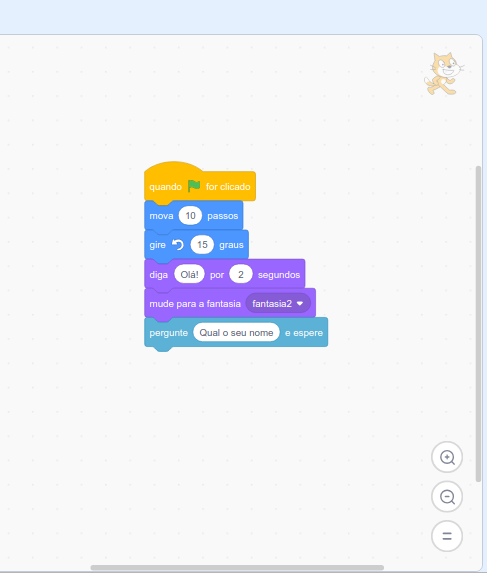
\includegraphics[height=7cm]{scratch3.png}
    \caption{Área de comandos do Scratch \label{scr3}}
    
\end{figure}

É nessa área que todas as programações são montadas como um puzzle.


A terceira área (\ref{scr4}) é onde se encontra o simulador do Ecrã (tela onde será projetada a programação), a relação dos atores e o palco com seus cenários.

\begin{figure}[h]

    \center

    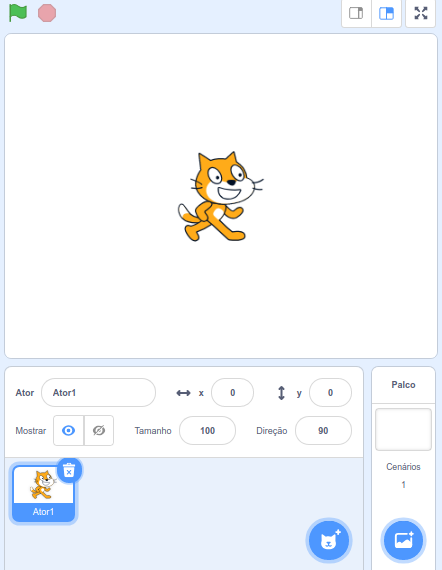
\includegraphics[height=7cm]{scratch4.png}
    \caption{Simulador de ecrã do Scratch \label{scr4}}
    
\end{figure}

O Ecrã é "mapeado" através de coordenadas cartesianas e o primeiro ator que aparece (um gato) se posiciona inicialmente no ponto (0,0), isto é, em x=0 e y=0 e o palco apresenta-se em branco.


Por ser uma linguagem de programação, toda ação deve ser dada na forma de comandos devidamente expressos nos seus blocos lógicos que são arrastados para uma área de comandos, conectados uns aos outros ou executados através de sub-rotinas ou de subdivisões. 
 
 As suas características de linguagem de programação e de um puzzle fazem com que o Scratch possa ser usado tanto como uma ferramenta para produção de Objetos de Aprendizagem como um meio de desenvolver o pensamento computacional do aluno e, em ambos os casos, esse uso poderá ser interdisciplinar. 

?colocar exemplos de objetos de aprendizagem e de desenvolvimento de pensamento computacional?

\chapter{Metodologia do curso}


%novas configurações

\bookmarksetup{startatroot}% 
% ---

% ---
% Conclusão
% ---

%\lipsum[31-33]

% ----------------------------------------------------------
% ELEMENTOS PÓS-TEXTUAIS
% ----------------------------------------------------------
\postextual

%---------------------------------------------------------------------
% INDICE REMISSIVO
%---------------------------------------------------------------------

%anexo de apendices
\begin{apendicesenv}
\partapendices

\chapter{Primeiro}

\end{apendicesenv}

%Linha na nova configuração

\printindex



\bibliography{bibliografia}

\end{document}